\chapter{Der neue Ansatz} \label{der-neue-ansatz}

\section{Steigende Robustheit durch TypeScript}

% Mehr Projekte nutzen TypeScript => sind bereits was Typing angeht robust
% TypeScript ist auch in fast allen IDEs integriert, also wird fast von jedem genutzt.
TypeScript verfügt, im Gegensatz zu JavaScript, über statische Typisierung. Dank der statischen Typisierung sind statische Typeanalysen und Operationen wie \textit{Go to Definition} und \textit{Go to Implementations} der Entwicklungsumgebungen (IDE) möglich. Diese Eigenschaften reduzieren Fehler im Zusammenhang mit falschen Typen erheblich. Wie in \ref{fig:js-und-ts-nutzung-2018-2024} abgebildet, wird TypeScript von immer mehr Entwicklern genutzt, während die JavaScript Nutzung abnimmt. \ref{fig:js-und-ts-nutzung-2018-2024} beinhaltet die tatsächliche Nutzung von TS nicht. Der TypeScript Compiler (tsc) ist in den meisten modernen IDEs, wie Visual Studio Code und den JetBrains IDEs wie IntelliJ IDEA und WebStorm integriert. Dies führt dazu, dass man auch beim JavaScript Code einige Vorteile von TypeScript bekommt.\cite{typeScriptDocumentary}

\begin{figure}[H]
  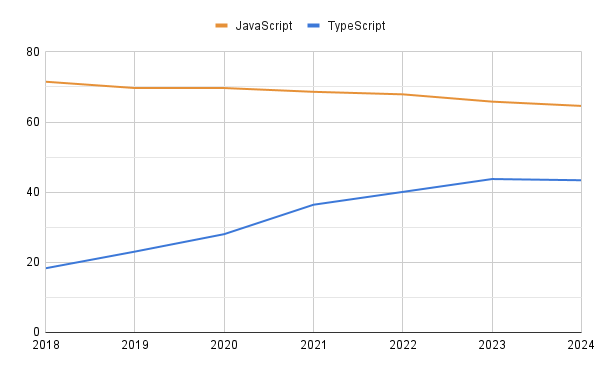
\includegraphics[width=0.85\textwidth]{js-und-ts-nutzung-2018-2024.png}
  \caption{Prozentuale Nutzung von JavaScript und TypeScript unter professionellen Entwicklern von 2018 bis 2024}
  \label{fig:js-und-ts-nutzung-2018-2024}
\end{figure}

% Um Implementierungsfehler zu vermeiden => Transitions robuster machen

\section {Unzureichende Robustheit in State-Management}

Der TypeScript-Faktor macht Webapplikationen, somit auch State-Management auf Typ-Ebene robuster und weniger fehleranfällig. Allerdings ist es für die Applikation immer noch möglich in einem falschen Zustand zu sein. Gegeben sei ein Redux Store, der für das Speichern einer Liste von \textit{items} zuständig ist. Definiert wird der Store wie folgt:

\begin{lstlisting}
  type FetchAction = {
    type: 'fetch'
  }

  type FetchSuccessfulAction = {
    type: 'fetch-successful',
    payload: Array<any>
  }

  type FetchFailedAction = {
    type: 'fetch-failed',
    payload: Error
  }

  type Action =
    | FetchAction
    | FetchSuccessfulAction
    | FetchFailedAction

  function reducer(
    state = { items: 'not-fetched' }, 
    action: Action
  ) {
    switch (action.type) {
      case 'fetch':
        return {
          ...state,
          items: 'fetching'
        }
      case 'fetch-successful':
        return {
          ...state,
          items: action.payload
        }
      case 'fetch-failed':
        return {
          ...state,
          items: action.payload
        }
      default:
        return state
    }
  }
  
  const store = createStore(reducer)
\end{lstlisting}

Es ist erlaubt, die \textit{FetchSuccessfulAction} Aktion zu versenden, ohne voher die \textit{Fetch} Aktion versendet zu haben. Das heißt: \q{\textit{items} wurden erfolgreich abrufen}, ohne die Anfrage zuvor gemacht zuhaben. Seitens Redux ist das Versenden einer Aktion immer, unbeachtet des aktuellen Zustandes, erlaubt. Dieser Faktor spricht gegen die Nachvollziehbarkeit und gilt für alle populäre SM Lösungen.

\section {Robustere Zustandsübergänge}

% State => Zustand
% Action => Übergang
% Reducer => Übergangsfunktion

Es wird vorgeschlagen den Applikationszustand wie ein Zustand eines DFAs zu behandeln. Im Falle von Redux werden die Aktionen als Übergänge und der Reducer als die Übergangsfunktion eines DFAs gesehen. Restliche Eigenschaften des Quintupels eines DFAs werden hierbei ignoriert.

Um die Übergangsfunktion zu definieren, wird pro Zustand eine \textit{Übergangsliste} aller Aktionen benötigt, die bei diesem Zustand erlaubt sind. Ein Problem hierbei ist allerdings, dass die Identifizierbarkeit der einzelnen Zustände nicht garantiert ist.
Abweichend von DFAs, sind die Zustände in Webapplikationen nicht immer serialisierbar. Nicht serialisierbare Objekte sind nicht immer identifizierbar. Im oberen Beispiel, sind die Zustände \textit{'not-fetched'} und \textit{'fetching'} vom Typ String und somit serialisierbar, allerdings sind die restlichen Zustände nicht serialisierbar (Zustand vom Typ Error und Array<any>). Um dieses Problem zu umgehen, wird eine \textit{Identitätsfunktion} emfohlen, um zwischen verschiedenen Zuständen zu unterscheiden. Sie akzeptiert als Paramter den aktuellen Zustand und gibt ein Boolean zurück.

\begin{lstlisting}
type IdentityFn<S> = (state: S) => boolean
\end{lstlisting}

% ODER SO:
% Sei $S$ die Menge aller Zustände und $B := \{true, false\}$, dann wird die \textit{Konfition Funktion} wie folgt definitiert:
% $f(s) = b | s \in S \land b \in B$

Mit dieser Funktion, kann der Anwender für die Indentifizierbarkeit der Zustände sorgen. Bei JavaScript Klassen, kann der \textit{instanceof} Operator genutzt werden, um auf die Instanz einer Klasse wie \textit{Error} zu prüfen.\cite{jsInstanceofOperator} Desweiteren, können bei Objekten auf eindeutige Eigenschaften, wie die Präzens eines Feldes per \textit{in} Operator geprüft werden.\cite{jsInOperator} Bei Arrays kann die \textit{Array.isArray} Funktion verwendet werden.\cite{jsIsArray} Durch die Kombinition dieser und weiteren Funktionen und Operatoren können weitere Datentypen und Fälle identifiziert werden.

Die \textit{Übergangsliste} lässt sich in einer Map wie folgt speichern:

\begin{lstlisting}
type TransitionMap<S extends IdentityFn<S>, A> = Map<S, Array<A>>
\end{lstlisting}

Für die \textit{Übergangsmap} gilt: \textit{Identitätsfunktion} ist der Schlüssel, während Liste von Aktionen der Wert ist.

In der Übergangsfunktion wird, der Zustandswechsel mit einer \textit{Validierungsfunktion} validiert. Diese prüft mit Hilfe der \textit{Übergangsmap} auf die Gültigkeit eines Übergangs und wirft einen Laufzeitfehler bei ungültigen Aufrufen. Falls der Übergang gültig ist, wirft sie keinen Fehler und der Zustandswechsel kann stattfinden. Der Laufzeitfehler sorgt dafür, dass der ungültige Aufruf berichtet wird und sich nicht zu einem langlebigen Bug entwicklen kann.

\subsection{Vorteile}

\begin{enumerate}
  \item \textbf{Übersichtlichkeit}: Damit die Validierung funktioniert, ist der Entwickler erzwungen die Übergangsmap definieren. So können fehlerhafte und überflüssige Übergänge schneller erkannt und korrigiert werden.
  \item \textbf{Erkennung von Bugs}: Bei fehlgeschlagener Übergangsvalidierung wird ein Laufzeitfehler geworfen, der über die Monitoringsysteme die Entwickler über einen Bug informieren kann. Ebenfalls möglich ist es, die falschen Übergänge lediglich zu loggen. Auf diesem Wege können die Entwickler ebenfalls über den Bug in Kenntnis gesetzt werden. Die letztere Strategie erlaubt jedoch im Worst-Case Weiterausführung falscher Geschäftslogik.
\end{enumerate}

\subsection{Nachteile}

\begin{enumerate}
  \item \textbf{Mehr Aufwand}: Damit der Ansatz funktioniert muss die Übergangsmap definiert werden. Diese Voraussetzung kostet zusätzliche Aufwand.
  \item \textbf{Erhöhte Ausfürungszeit}: Außerdem erhöht sich Ausführungszeit der gesamten Applikation durch die Validerung bei jedem Zustandswechsel. Diese hinzukommende Zeit ist jedoch zuvernachlässigen, wenn die Identitätsfunktion effizient ist und keine Nebeneffekten erzeugt, also eine \textit{pure function} ist.
\end{enumerate}
